\section{Experiments}
\label{sec:experiments}
\subsection{Kernel Ridge Regression}
\begin{figure}
\centering
\begin{tabular}{c c}
	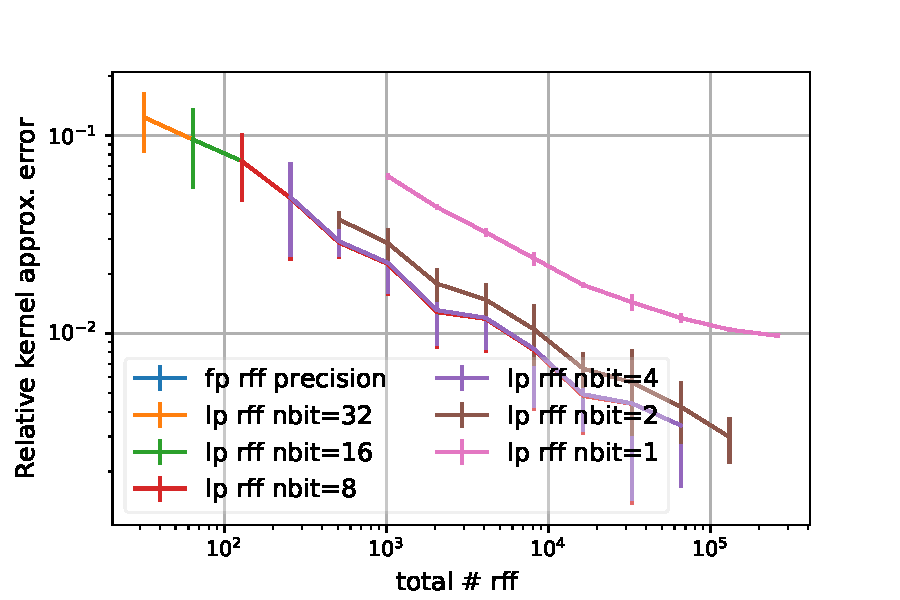
\includegraphics[width=.45\linewidth]{figures/kernel_approx_error_n_fp.pdf} &
	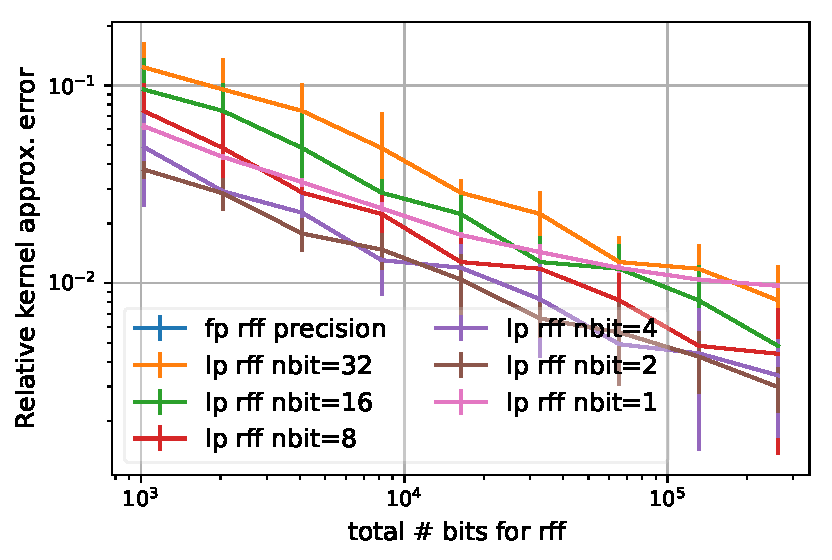
\includegraphics[width=.45\linewidth]{figures/kernel_approx_error.pdf} \\
	(a) & (b) \\
	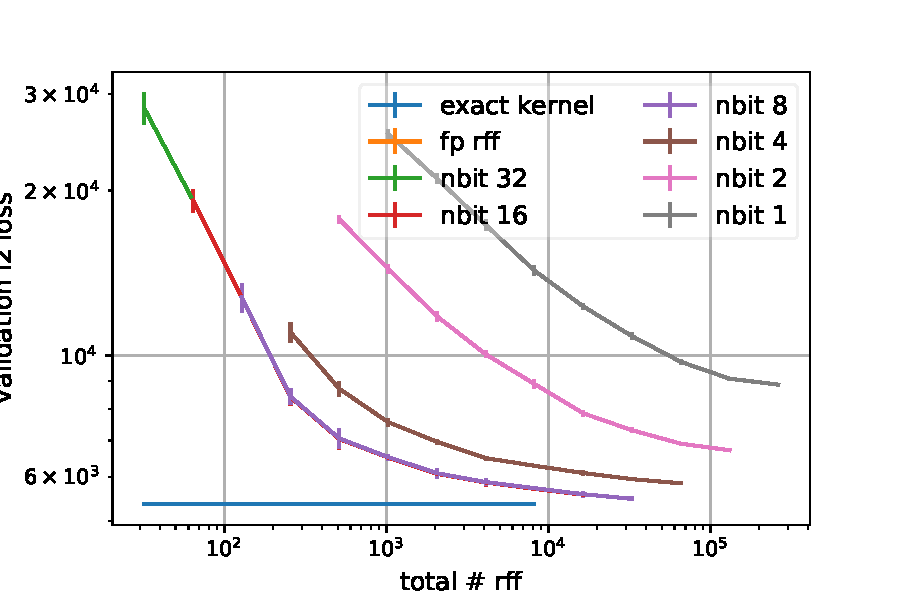
\includegraphics[width=.45\linewidth]{figures/valid_l2_n_fp.pdf} &
	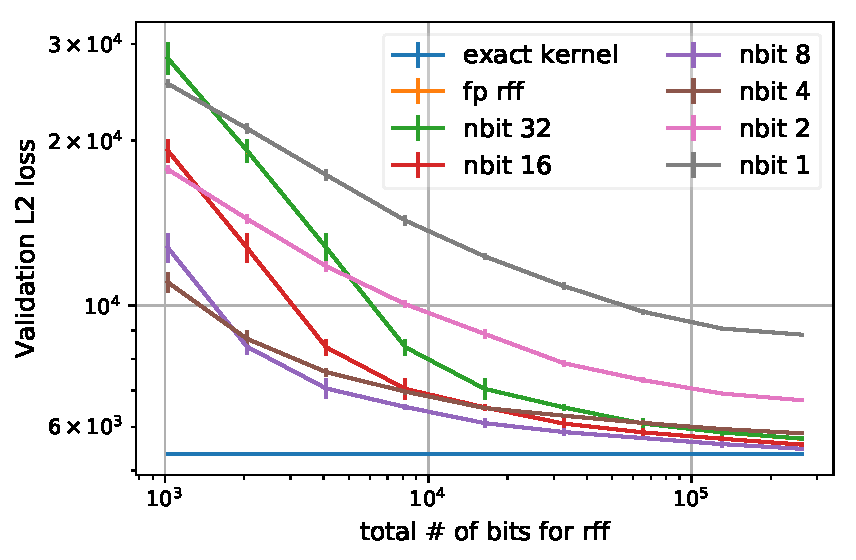
\includegraphics[width=.45\linewidth]{figures/valid_l2.pdf}  \\
		(c) & (d) \\
\end{tabular}
%\begin{tabular}{c c}
%	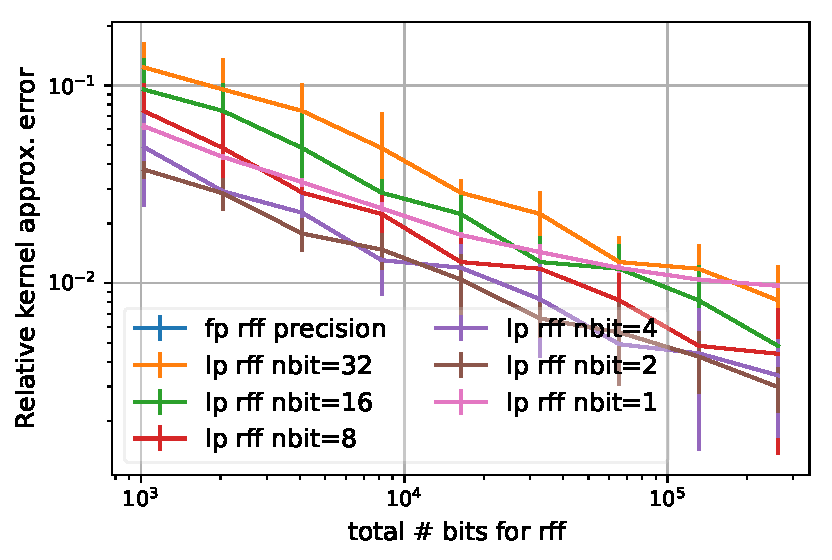
\includegraphics[width=.45\linewidth]{figures/kernel_approx_error.pdf} &
%	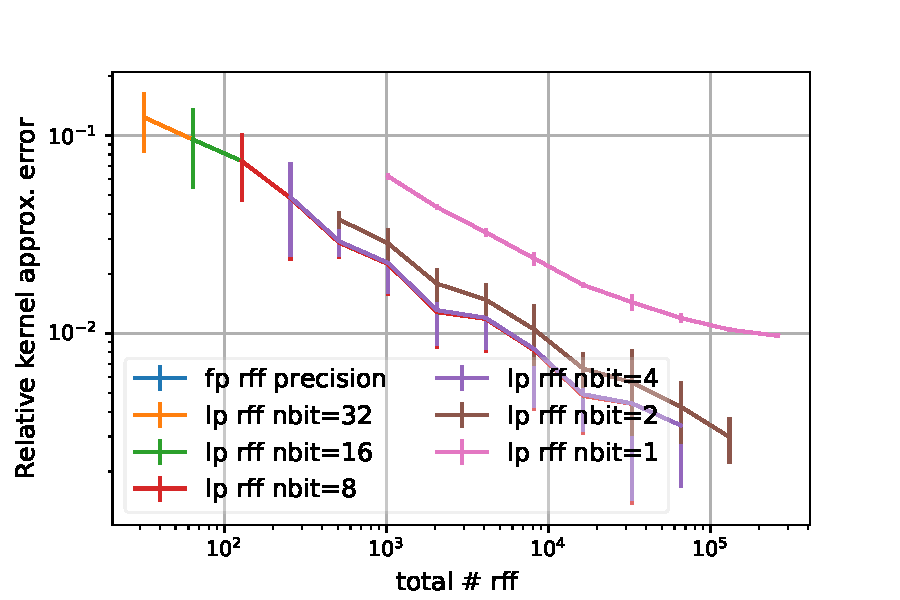
\includegraphics[width=.45\linewidth]{figures/kernel_approx_error_n_fp.pdf} \\
%	(a) & (b) \\
%	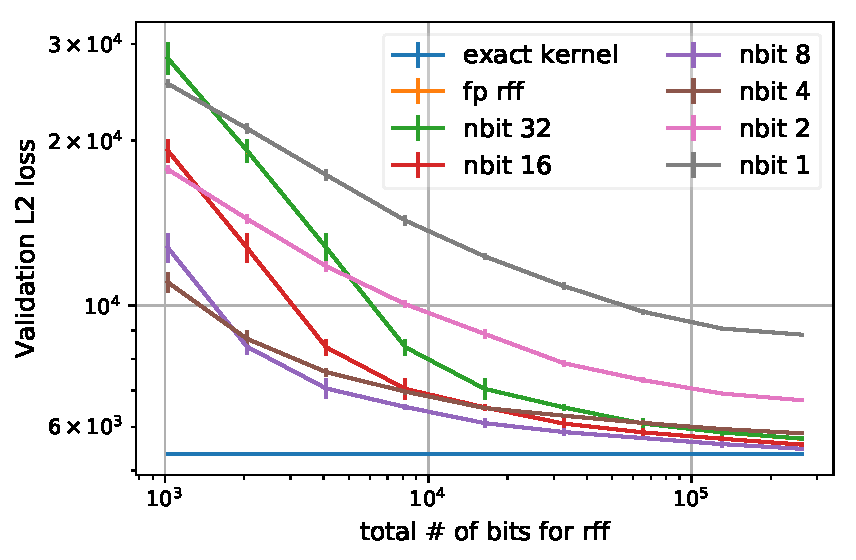
\includegraphics[width=.45\linewidth]{figures/valid_l2.pdf} &
%	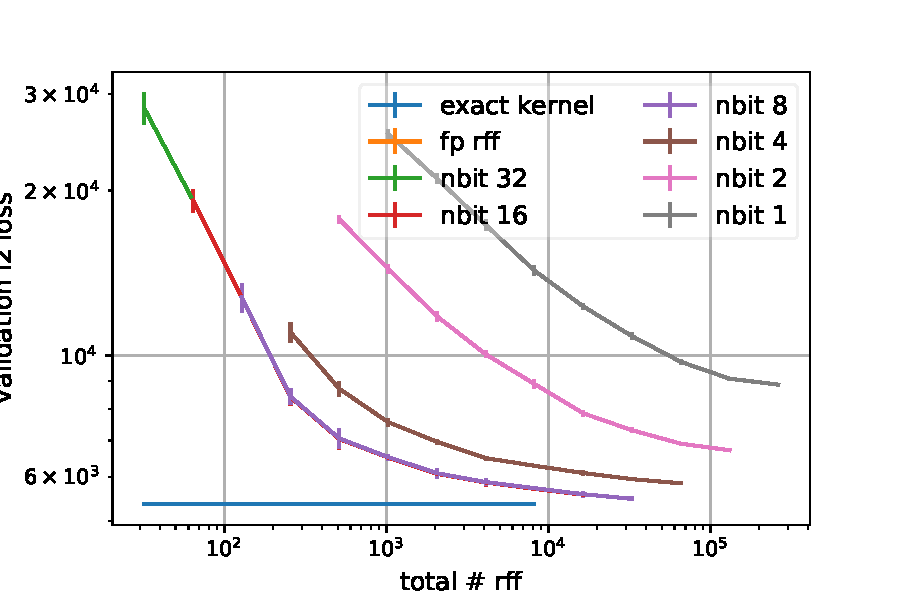
\includegraphics[width=.45\linewidth]{figures/valid_l2_n_fp.pdf}  \\
%		(c) & (d) \\
%\end{tabular}
\caption{Kernel approximation and validation L2 loss for Kernel Ridge Regression on UCI Census dataset. (a) and (c) compare different precision representation with the same number of random Fourier features. (b) and (d) compare different precision representation under same memory bits budgets.}
%\caption{Kernel approximation and validation L2 loss for Kernel Ridge Regression on UCI Census dataset. (a) and (b) compare different precision representation under same memory bits budgets. (c) and (d) compare different precision representation with the same number of random Fourier features.}
\label{fig:kernel_and_l2}
\end{figure}

We use UCI Census dataset for the experiments on kernel ridge regression. This dataset contains 16k training samples with 119 original features. Besides from reporting the kernel approximation errors, we also report the validation L2 loss in the regression problem. The reported L2 loss for each feature precision is from a grid search over $\{1e^{-6}, 1e^{-5}, ..., 1e^{-1}, 1, 10, 100\}$ for L2 regularizer strength $\lambda$. To report statistically meaningful results, we average the performance metrics from 5 random seeds for random Fourier feature generation and stochastic quantization. We uniformly use Gaussian kernels with $\sigma=30.0$ for our experiments on kernel ridge regression.

\subsubsection{Kernel approximation error and validation L2 loss}
In this section, we evaluate low precision random Fourier features in comparison to full precision features. We report the kernel approximation error and regression performance (the validation L2 loss on the heldout dataset) when using (1) the same number of random Fourier features and (2) using the same memory budget for random Fourier features.
As shown in Figure~\ref{fig:kernel_and_l2} (a) and (c), when using the same number of random Fourier features, we observe the kernel approximation error only degrades when using 1 or 2 bits; the low precision representation in other precision level is on par with the full precision features. Regarding the regression performance, i.e. the validation l2 loss, we only observe degradation for 1,2 and 4 bits representation.
%the kernel approximation error keeps decreasing from full precision to 2 bits representation, while validation L2 loss only starts to observably degrade after the precision gets lower than or equal to 4 bits. For precision using 8 bits or higher number of bits, the validation L2 loss closely overlap with the ones from full precision random Fourier features. 
Furthermore, in~\ref{fig:kernel_and_l2} (b) and (d), we compare the performance of feature representation in different precision \emph{under the same memory bits budget for each data sample}. In this setting, we observe 2 or 4 bit features presents the best kernel approximation error, while 8 bits representation gives the best validation L2 loss.
%Kernel methods based on RFF typically improves when more RFF presents, while more precise feature representation can demonstrate lower approximation error. \emph{Indeed, under the memory budgets, we observe a trade-off between the number of RFF and the representation precision of RFF in~\ref{fig:kernel_and_l2}(a) and (b). Specifically, under different memory budget for the RFF representation of each data sample, 2 or 4 bits representation presents the best kernel approximation, while 8 bits demonstrates the best validation L2 loss consistently.}

%\begin{figure}
%	\centering
%	\begin{tabular}{c c}
%		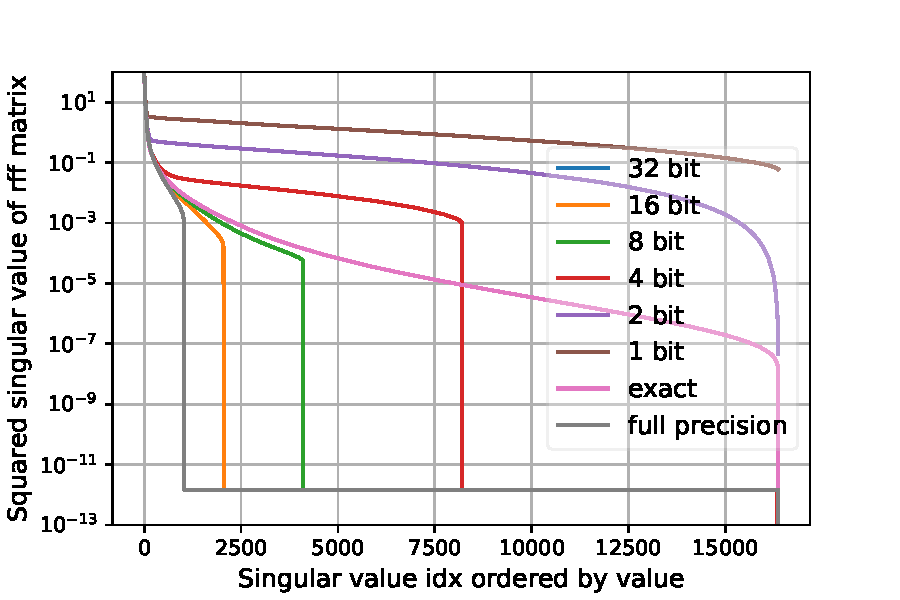
\includegraphics[width=.45\linewidth]{figures/spectrum_1024.pdf} &
%		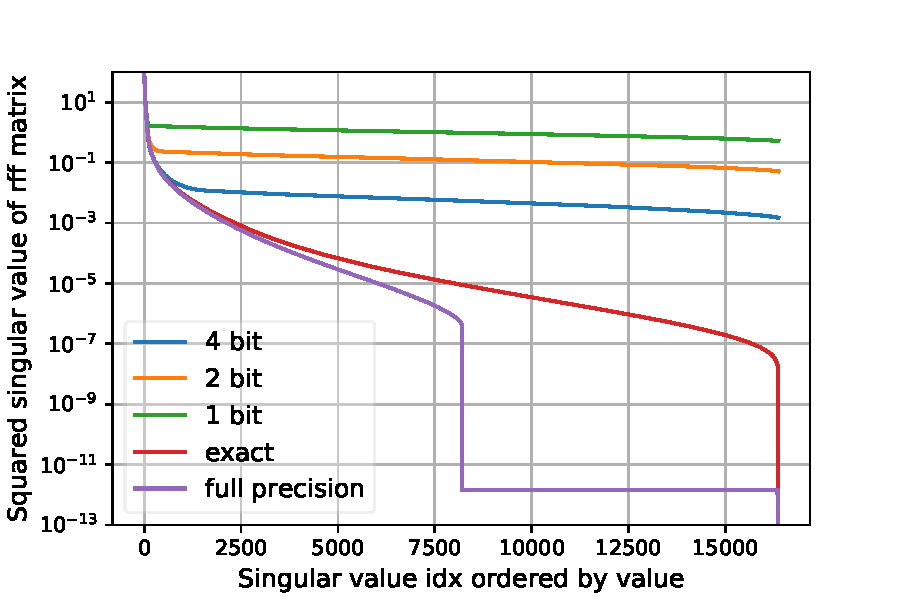
\includegraphics[width=.45\linewidth]{figures/spectrum_8192.pdf}  \\
%		(a) & (b) \\
%		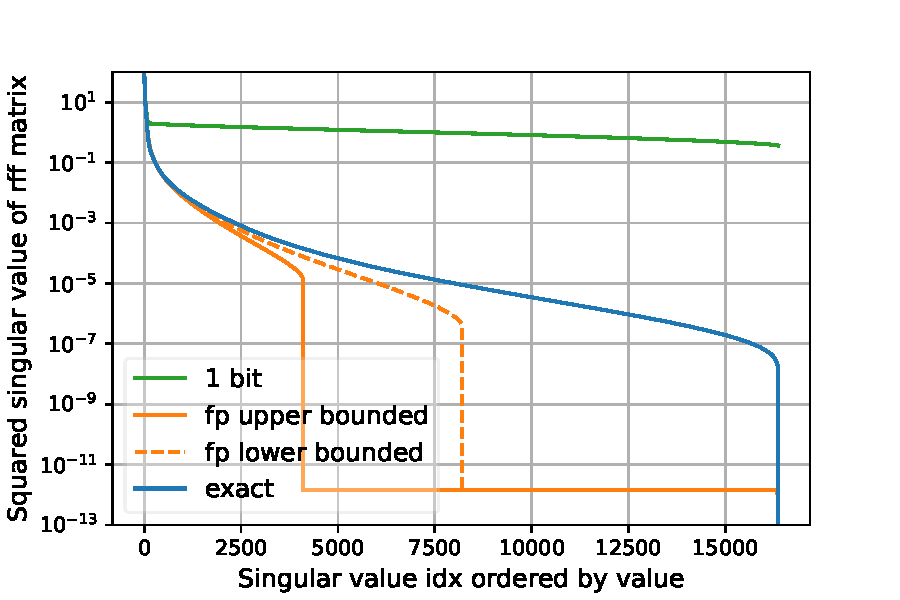
\includegraphics[width=.45\linewidth]{figures/different_spectrum_with_same_kernel_approx_error_log.pdf} &
%		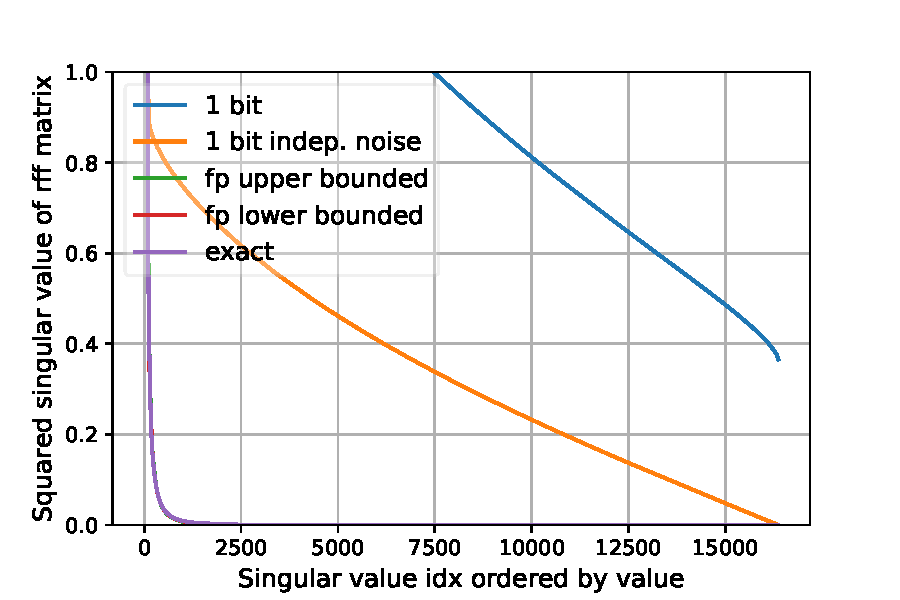
\includegraphics[width=.45\linewidth]{figures/different_spectrum_with_same_kernel_approx_error.pdf}\\
%		(c) & (d)
%	\end{tabular}
%	\caption{Spectrum (eigen values) of the kernel matrix. The spectrums from different precision representation are shown under a) 3.2k (equivalent to 1024 full precision rffs) and b) 25.6k bits memory budget (equivalent to 8192 full precision rffs) for the feature of each sample. (c) Configurations with similar approximation errors can demonstrate very different spectrum; we compare the 1 bit representation to the full precision configurations giving 1) the highest approx. error that is lower than the 1 bit configuration 2) the lowest approx. error that is higher than the 1bit configuration. (c) Replot (b) in decimal scale to visualize the difference of spectrums; the spectrums from kernel matrix using 1) a single stochastic quantization and 2) two independent stochastic quantization for the feature matrix and its transpose. \emph{Note in (c) and (d), we can observe independent quantization for RFF matrix and its transpose (indep. noise curves in the figures) presents spectrum closer to the exact kernel than using the same stochastic quantization for RFF matrix and its transpose.} }
%	\label{fig:spectrums}
%\end{figure}

\subsubsection{Spectrum of kernel matrix correlates with L2 loss}
\label{subsubsec:bump_spectrum}
\begin{figure}
	\centering
	\begin{tabular}{c c}
		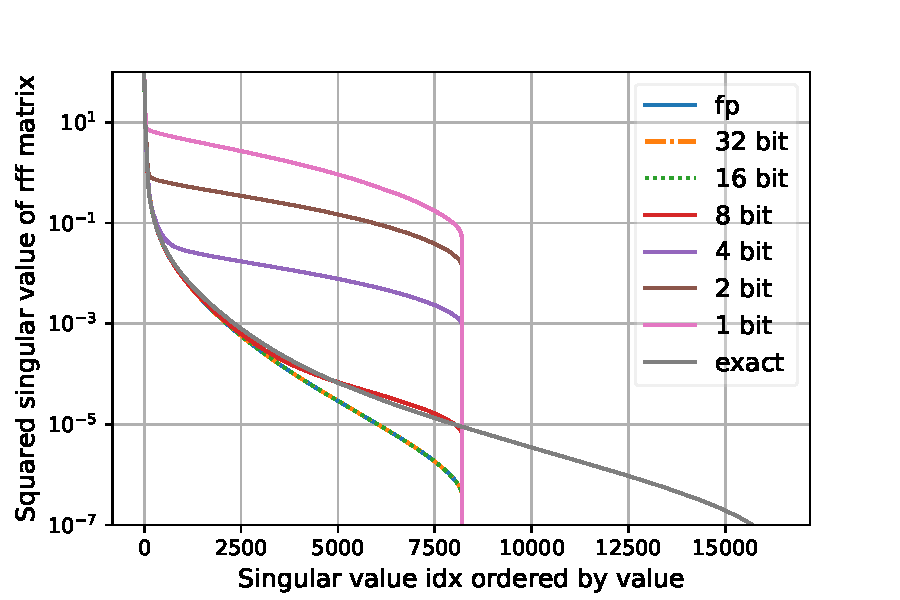
\includegraphics[width=.45\linewidth]{figures/spectrum_n_rff_8192.pdf} &
		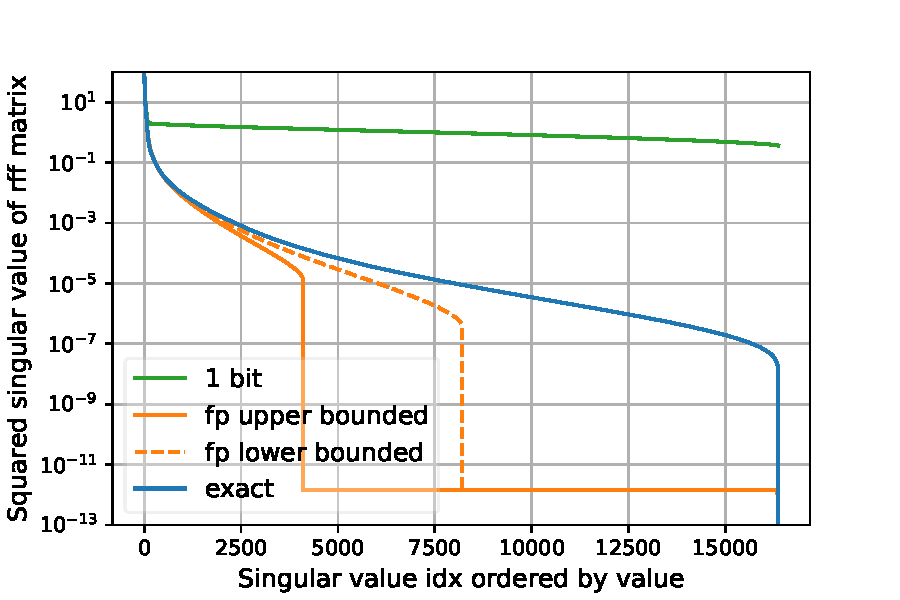
\includegraphics[width=.45\linewidth]{figures/different_spectrum_with_same_kernel_approx_error_log.pdf} \\
%		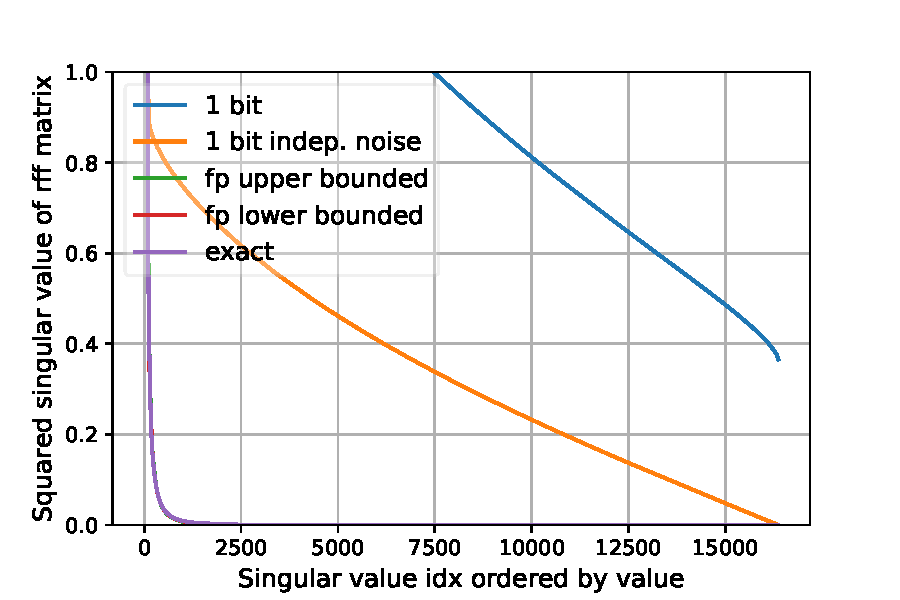
\includegraphics[width=.33\linewidth]{figures/different_spectrum_with_same_kernel_approx_error.pdf}\\
		(a) & (b) %& (c)
	\end{tabular}
	\caption{Spectrum (eigen values) of the kernel matrix. (a) The spectrums from different precision representation is shown under 8192 random Fourier features. (b) Configurations with similar approximation errors can demonstrate very different spectrum; we compare the 1 bit representation to the full precision configurations giving 1) the highest approx. error that is lower than the 1 bit configuration 2) the lowest approx. error that is higher than the 1bit configuration.}
	\label{fig:spectrums}
\end{figure}

In our theory in Section~\ref{sec:spectrum}, we have been discussing how low precision introduce quantization variance, which results in bumping up the spectrum of kernel matrix. To empirically support our analysis on the spectrums, in Figure~\ref{fig:spectrums} (a), we demonstrate the kernel matrix spectrum from 8192 random Fourier features in different precision. 
More specifically, we approximate the kernel matrix with $\bm{K}'=\tilde{\bm{Z}}\tilde{\bm{Z}}^T$ where $\tilde{\bm{Z}}=Q(\bm{Z})$ is the quantized version of random Fourier feature $\bm{Z}$. This quantization approach corresponds to the case where $\bm{K}'=(\bm{Z} + \bm{C})(\bm{Z} + \bm{C})^T$ in Section~\ref{sec:spectrum}; it imposes the same noise on the feature matrix $\bm{Z}$ and its transpose.
%Note in this section, we discuss the case where the feature matrix and its transpose are quantized to the same value on the corresponding entries. 
We can observe 8, 16 and 32 bits representation has spectrums close to the spectrum of full precision RFF kernel matrix. However, for 4, 2 and 1 bits representation has significantly higher spectrums than 8, 16 and 32 bits representation. Remember that in Figure~\ref{fig:kernel_and_l2}, we have seen 8, 16 and 32 bits representation demonstrates similar L2 loss, while 4, 2 and 1 bits can show observably worse performance. \emph{From these observations, we believe spectrum is closely correlated with the validation L2 loss. Indeed if the two RFF kernel matrices has the same spectrum, the RFF features matrices are only different up to rotation and flipping; the spectrum are at the heart of the generalization performance for the kernel ridge regression model. We refer to Section \ref{sec:fixed_design} for more detailed discussion on generalization performance and spectrum, in the context of ``fixed design'' kernel ridge regression.} 

Additionally, we compare to the correlation between kernel approximation error and lO2 loss, to further emphasize the strong correlation between spectrum and L2 loss. In Figure~\ref{fig:spectrums} (b), we demonstrates the spectrums from 3 configurations with very similar kernel approximation error. Specifically, we compare 1 bit RFF with 131k features to two full precision RFF configuration with the closest kernel approximation error; these 2 full precision configurations respectively gives 1) the highest approx. error that is lower than the 1 bit configuration (8192 features) 2) the lowest approx. error that is higher than the 1bit configuration (4096 features). The 3 configurations shows close relative kernel approximation error around $1e^{-2}$, but can demonstrate very different spectrum in Figure~\ref{fig:spectrums} and very different validation L2 loss in Figure~\ref{fig:kernel_and_l2} (d).

\subsubsection{Effect of independent quantization of RFF matrix and its transpose}
In Section~\ref{subsubsec:bump_spectrum}, we have validated the analysis in Section~\ref{sec:spectrum}, empirically showing low precision RFF bumps up the kernel matrix spectrum. The discussion in Section~\ref{sec:spectrum} also suggested a technique to reduce the height of the bump. Specifically, we can approximate the kernel matrix $\bm{K}'=\tilde{\bm{Z}}_1\tilde{\bm{Z}}_2^T$ where $\tilde{\bm{Z}}_1$ and $\tilde{\bm{Z}}_1$ are two independent instantiations of stochastic quantization (i.e. quantization noise matrices $\bm{C}\neq \bm{D}$ in Section~\ref{sec:spectrum}).
We compare this quantization approach to the basic case in Section~\ref{subsubsec:bump_spectrum} where the low precision kernel approximation $\bm{K}'=\tilde{\bm{Z}}\tilde{\bm{Z}}^T$ uses a single instantiation of stochastic quantization. In Figure~\ref{fig:indep_quant}, we show the comparison under two different memory bits budgets for the feature of each sample. In both the budgets, the spectrum becomes significantly lower after switching to independent quantization for RFF matrix and its transpose. The also observe that, when using two independent instantiations of stochastic quantization, the spectrum from 8192 features is significantly lower than the one from 1024 features. This aligns with the implication from the theory in Section~\ref{sec:spectrum}: the more features we have in the low precision representation, the lower the spectrum will be.
%Given two kernel function $k(\cdot, \cdot)$ and $k'(\cdot, \cdot)$, we assume the prediction on datum $x$ using $k$ and $k'$ are $h(x)$ and $h'(x)$ respectively. The prediction difference $|h(x) - h'(x)|$ has an upper bound involving two quantities $\| \bm{K} - \bm{K}' \|_2$ and $\| \bm{k}_x - \bm{k}_x' \|$ [3]; in this bound, $\bm{K}$ and $\bm{K}'$ are the training data kernel matrices, while $\bm{k}_x$ and $\bm{k}'_x$ are the test kernel values (i.e. kernel values between test sample $x$ and training samples). In this section, we evaluate a simple technique to reduce $\| \bm{K} - \bm{K}' \|_2$. We continue to discuss the influence of $\| \bm{k}_x - \bm{k}_x' \|$ in Section~\ref{subsubsec:test_var_reduce}.


\subsubsection{Effect of reducing variance in test sample features}
\label{subsubsec:test_var_reduce}
In Section~\ref{sec:reduce_test_noise_theory}, we discuss that reducing noise on test sample features can improve regression performance, i.e. the validation L2 loss in kernel ridge regression. 
%Given two kernel function $k(\cdot, \cdot)$ and $k'(\cdot, \cdot)$, we assume the prediction on datum $x$ using $k$ and $k'$ are $h(x)$ and $h'(x)$ respectively. The prediction difference $|h(x) - h'(x)|$ has an upper bound involving two quantities $\| \bm{K} - \bm{K}' \|_2$ and $\| \bm{k}_x - \bm{k}_x' \|$ [3]; in this bound, $\bm{K}$ and $\bm{K}'$ are the training data kernel matrices, while $\bm{k}_x$ and $\bm{k}'_x$ are the test kernel values (i.e. kernel values between test sample $x$ and training samples).
%To preliminary validate the influence of $\| \bm{k}_x - \bm{k}_x' \|$ on prediction error of low precision kernel regressor, 
To preliminarily validate this effect, we first train the kernel ridge regression model with low precision RFF. In the test phase, we evaluate the validation L2 loss using prediction $\hat{y}=\bm{w}^T\bm{z} + b$, where we use \emph{full precision} test sample RFF instead of its quantized low precision version; we call this approach as variance reduction technique. We compare this variance reduction technique to the basic case where the model predicts with $\tilde{\hat{y}}=\bm{w}^T\tilde{\bm{z}} + b$ using quantized low precision test sample RFF $\tilde{\bm{z}}$. In Figure~\ref{fig:var_reduction}, by using the variance reduction technique, we can significantly improve the validation L2 loss for models trained using 1, 2 and 4 bits low precision RFF. Noticeably, with variance reduction technique, 4 bit representation can outperform 8 bit representation in low memory budget, while 8 bit representation is consistently the best for validation L2 loss when we do not use the variance reduction technique.

We can also understand the variance reduction technique in another perspective. Given two kernel function $k(\cdot, \cdot)$ and $k'(\cdot, \cdot)$, we assume the prediction on datum $x$ using $k$ and $k'$ are $h(x)$ and $h'(x)$ respectively. The prediction difference $|h(x) - h'(x)|$ has an upper bound involving two quantities $\| \bm{K} - \bm{K}' \|_2$ and $\| \bm{k}_x - \bm{k}_x' \|$ [3]; in this bound, $\bm{K}$ and $\bm{K}'$ are the training data kernel matrices, while $\bm{k}_x$ and $\bm{k}'_x$ are the test kernel values (i.e. kernel values between test sample $x$ and training samples).
Our empirical observation validates the importance of $\| \bm{k}_x - \bm{k}_x' \|$ in bounding the prediction error of a low precision RFF kernel regressor, when comparing to the prediction of a full precision RFF kernel regressor. 


\begin{figure}
	\centering
	\begin{tabular}{c c}
		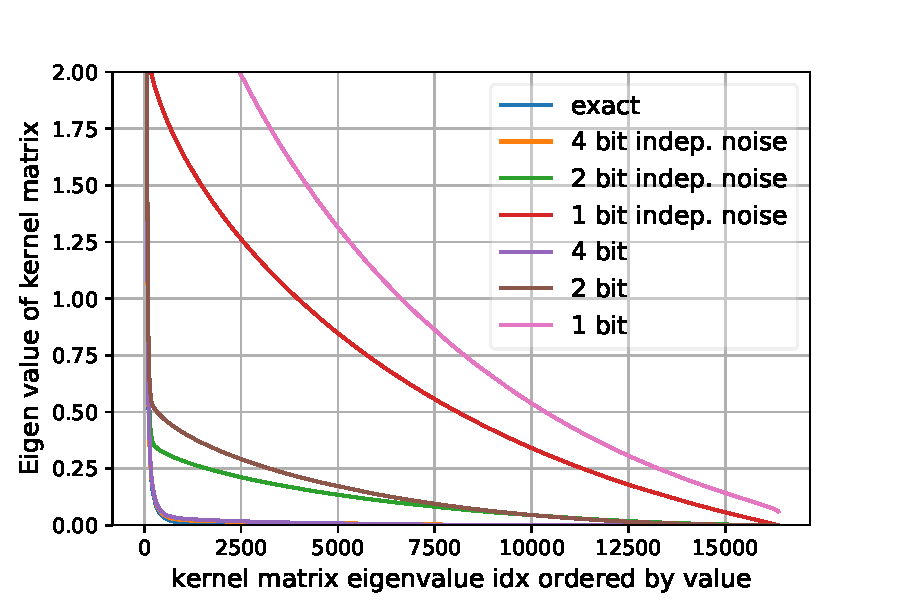
\includegraphics[width=.45\linewidth]{figures/spectrum_1024_indep.pdf} &
		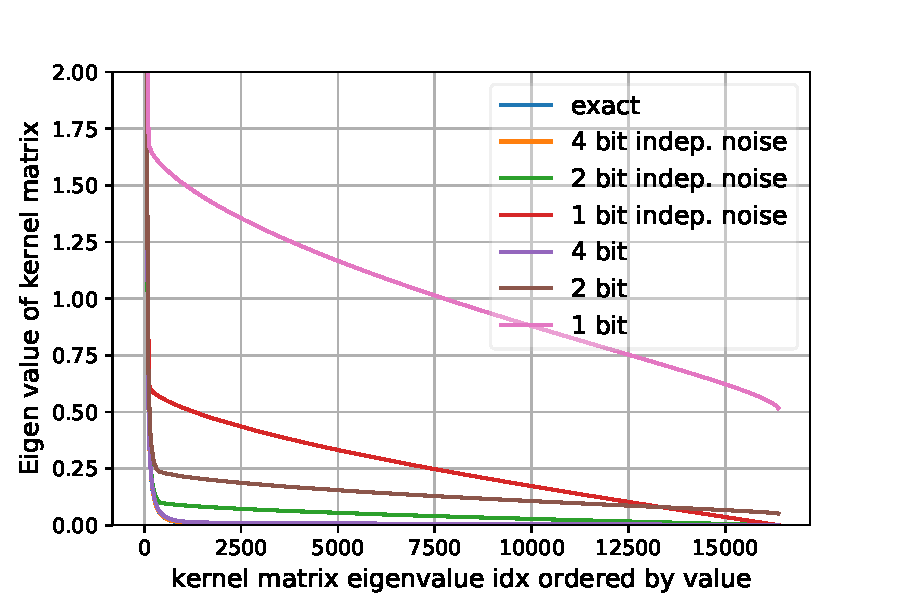
\includegraphics[width=.45\linewidth]{figures/spectrum_8192_indep.pdf} \\
		(a) & (b) \\
		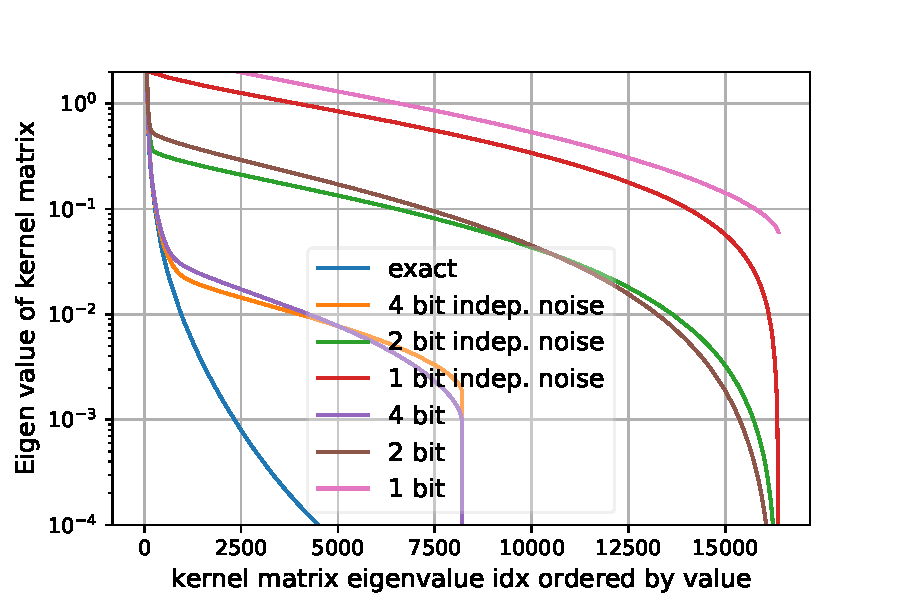
\includegraphics[width=.45\linewidth]{figures/spectrum_1024_indep_log.pdf} &
		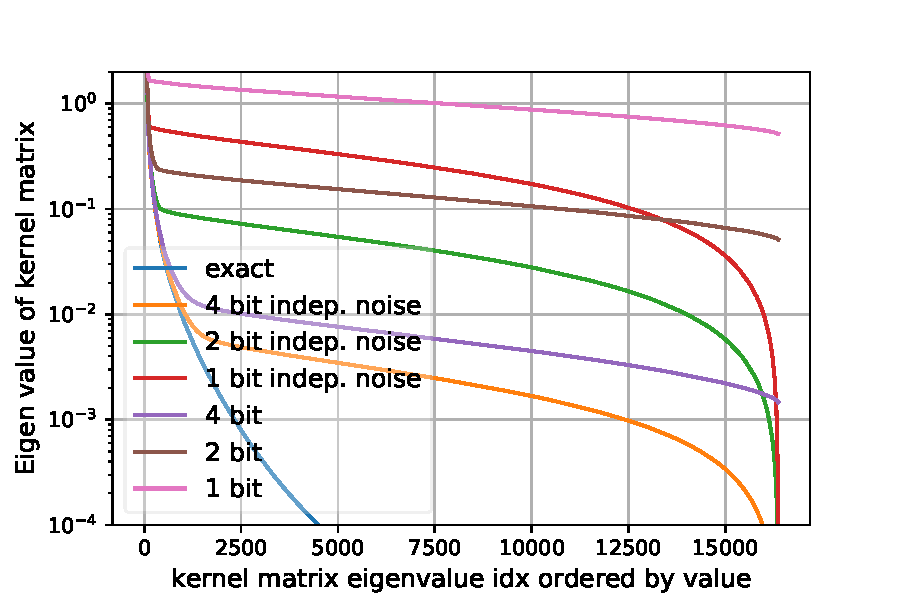
\includegraphics[width=.45\linewidth]{figures/spectrum_8192_indep_log.pdf} \\
		(c) & (d)
	\end{tabular}
	\caption{Spectrum (eigen values) of the kernel matrix. (a) The spectrum from different precision representation under 32k bits memory budget (1024 full precision rffs) for the feature of each sample. (b) The spectrum from different precision representation under 25.6k bits memory budget (1024 full precision rffs) for the feature of each sample. (c) and (d) is re-visualization of (a) and (b) in log-scale; it zooms in small value regions.}
	\label{fig:indep_quant}
\end{figure}


\begin{figure}
	\centering
	\begin{tabular}{c c}
		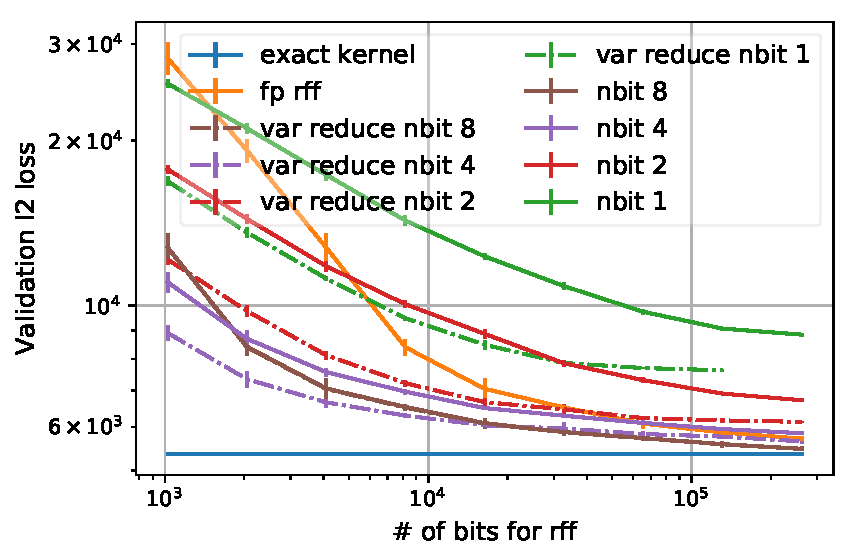
\includegraphics[width=.45\linewidth]{figures/valid_l2_var_reduction.pdf} &
		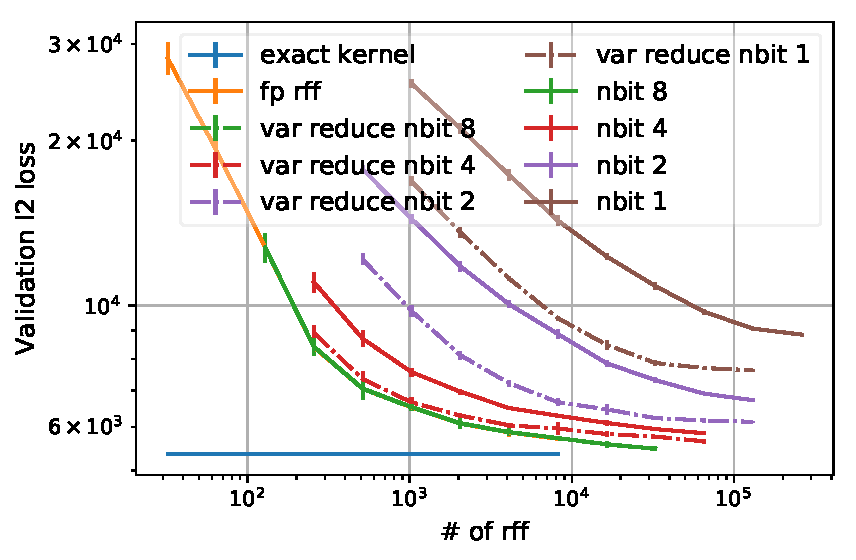
\includegraphics[width=.45\linewidth]{figures/valid_l2_n_fp_var_reduction.pdf} \\
		(a) & (b)
	\end{tabular}
	\caption{We train with low precision RFF and test with full precision RFF. Though the model is trained with low precision features, the test L2 loss can be improved by reducing variance in test RFF. (a) compare different precision representation under same memory bits budgets. (b) compare different precision representation with the same number of random Fourier features. }
	\label{fig:var_reduction}
\end{figure}

%
%512 2 bits, 4096 fp 8192 fp, 4096 1 bit

